
\documentclass{article}
\usepackage{graphicx}

\setlength{\parindent}{0pt}
\setlength{\parskip}{0.2cm}
\topskip 0.0in
%\pagestyle{empty}

\begin{document}
\title{CS8803: STR, Spring 2016. \\Lab 1: Robot Localization Report}
\author{
  Bhavishya Mittal, Sumant Hanumante, Sai Teja Duthuluri\\
  \texttt{(bmittal6, shanumante3, dst3)} @gatech.edu
}

\date{\today}

\maketitle

\section{Introduction}
This lab assignment problem is based on robot localization and particle filtering. Given the layout of a map along with odometry and laser finder readings from a robot, the aim is to accurately find the location of the moving robot in the map.

\section{Approach}
The basic approach of localizing a robot in the map (map already given) is through using particle filters.
\begin{enumerate}
 \item Generate a cache of the ray-casting data on map for future use: In this cache, the map is divided into grid cells and for each unoccupied grid cell, the distance to the nearest obstacle is calculated along angles 10 degrees apart in the range 0 to 360 degrees.
 \item Initialize a sensor model: This involves caching a matrix which has the dimensions of \textit{max\_sensor\_range} x \textit{max\_sensor\_range} and contains the probability values for actual sensor value, given the expected sensor value. These values are computed using $p_{hit}$, $p_{short}$, $p_{max}$ and $p_{rand}$ PDFs.
 \item Randomly sample particles over all unoccupied locations in the map pointing in random directions.
 \item Read in the odometry and laser finder readings from the log file. We consider only the laser sensor readings and take odometer data from it. To avoid taking multiple readings at same location, we take the next laser reading only if the robot has moved considerably (atleast 2dm) compared to previous reading.
 \item Run the particle filter algorihm.
 \item For every reading, we take each particle and sample from the motion model to get the new particle position. 
 \item We have the sensor values from the reading and we get the expected sensor values for this newly sample particle from the already cached ray-casted data. Run the sensor model on this to get the weight for each newly sampled particle.
 \item Resample the particles based on their weight.
 %\item Resample on two occasions: when the number of particles in the system is too less (20\% of the initial quantity) or after a random time interval.
 \item Repeat steps $\left(5-8\right)$ for all log file readings.
\end{enumerate}

\section{Implementation}
\subsection{Motion Model}
For our motion model, we consider the \textit{Odometry Motion Model} that uses odometry data as given in textbook. And since we are using particle filters, we use the sampling approach to model the motion of the robot. We repeatedly sample (max\_retries = 20) for a new particle until it lies in an unoccupied region of the map. If we do not get such a particle, we explicitly set the weight to 0. This motion model has a number of tunable parameters which have been discussed in a section below.

\subsection{Sensor Model}
For our sensor model, we follow the basic algorithm for beam models of range finders, as given in textbook. Here, our model is an aggregation of four PDFs: $p_{hit}$, $p_{short}$, $p_{max}$ and $p_{rand}$. Each of these four PDFs have a corresponding weight, speicifed by $z_{hit}$, $z_{short}$, $z_{max}$ and $z_{rand}$. Given a pose reading, we calculate the expected odometry reading using ray casting method. This is done for every particle. The tuning of the \textit{z} parameters is discussed in a section below.

%\subsection{Sampling Distribution}
%For any two successive poses (odometry readings), we calculate the estimated next pose using the \textit{Sampling Odometry Motion Model}. Using this estimated pose, we check the corresponding probability in probability map that we had generated using the map in the beginning. If this probability is greater than zero, then we find the weight of this probability using the sensor model. INSERT TEXT HERE!!!

%\pagebreak

\subsection{Resampling Procedure}
We resample particles based on their weights. We first normalize the weights and then align them sequentially from 0 to 1. Then, we sample a number in range 0 to 1 from a uniform distribution and select the particle corresponding to the weight where this number falls. This way, we resample all the particles again. Some modification is done to this resample step to solve robot kidnap problem. This modified version is explained in extra credit section.

\section{Parameter Tuning}
\subsection{Motion Model}
The motion model consists of four parameters: $\alpha_{1}$, $\alpha_{2}$, $\alpha_{3}$ and $\alpha_{4}$.

The parameters $\alpha_{1}$ and $\alpha_{2}$ are used to calculate the difference in rotation angle between the estimated and actual robot pose. We do not want this difference to be more than $5\,^{\circ}$. Based on this limit, we tuned the two parameters so that this difference would always be less than $5\,^{\circ}$. We have $\alpha_{1} = \alpha_{2} = 0.005$.

We perform the same procedure for tuning $\alpha_{3}$ and $\alpha_{4}$, which are used to calculate the difference in translation between estimated and actual robot pose. We want the difference to be less than 1dm in this case. After tuning, the best results were obtained for $\alpha_{3} = \alpha_{4} = 0.12$.

\subsection{Sensor Model}
The sensor model consists of six parameters. Four for the weight of prabability functions : $z_{hit}$, $z_{short}$, $z_{max}$ and $z_{rand}$ and two $\sigma$ and $\lambda$ for normal and exponential distribution repectively. The 4 weight parameters were tuned by looking at the PDF curve and observing the corresponding behaviour in the actual map. We set $\sigma = 2$ as we assume that expected sensor reading and observed reading should not be more than 2dm apart. $\lambda$ was set empirically. Some of the PDF curves have been presented in the Results section below.

\pagebreak

\section{Results}

\subsection{Map Model}
Given below is a image of the map generated from the cached ray tracing data. We used this to validate our sensor model
is working as expected.

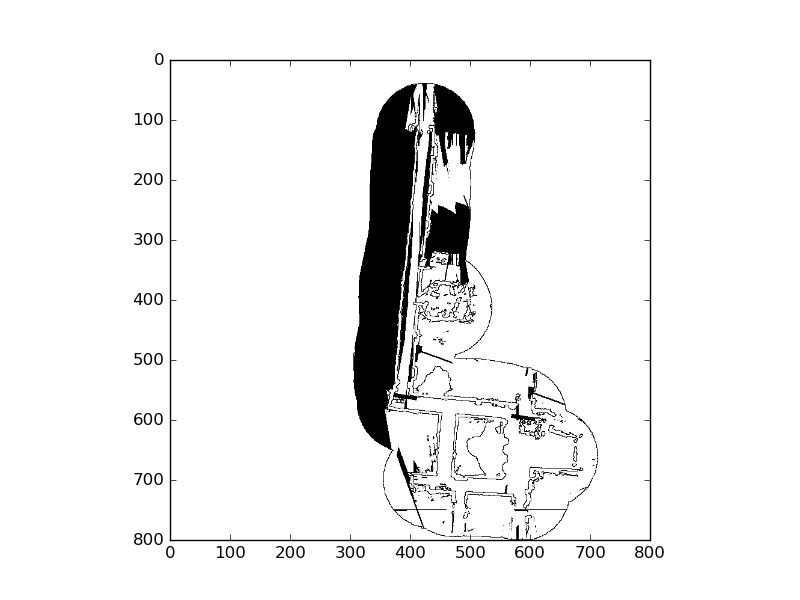
\includegraphics[width=\textwidth]{map1}

\pagebreak

\subsection{Sensor Model}
Given below are a few plots of the sensor models used in our code.

\begin{figure}[!hb]
 \centering
 \begin{minipage}[b]{0.4\textwidth}
  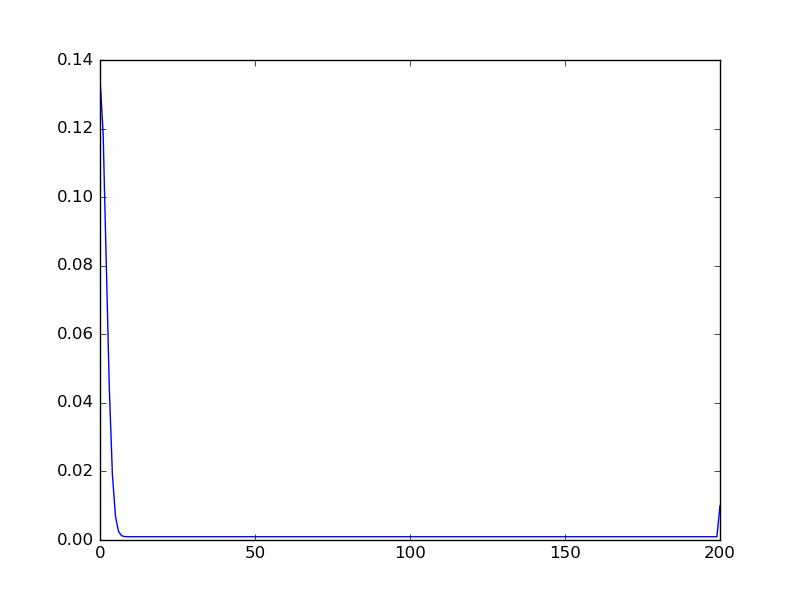
\includegraphics[width=\textwidth]{sensor_model_1.png}
  \caption{Mean 0}
 \end{minipage}
 \hfill
 \begin{minipage}[b]{0.4\textwidth}
  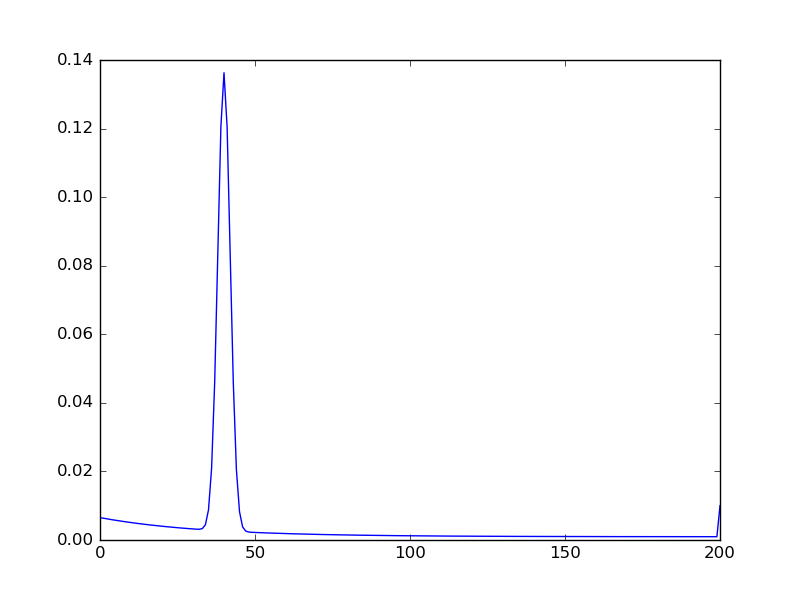
\includegraphics[width=\textwidth]{sensor_model_3.png}
  \caption{Mean 40}
 \end{minipage}
 \vfill
 \begin{minipage}[b]{0.4\textwidth}
  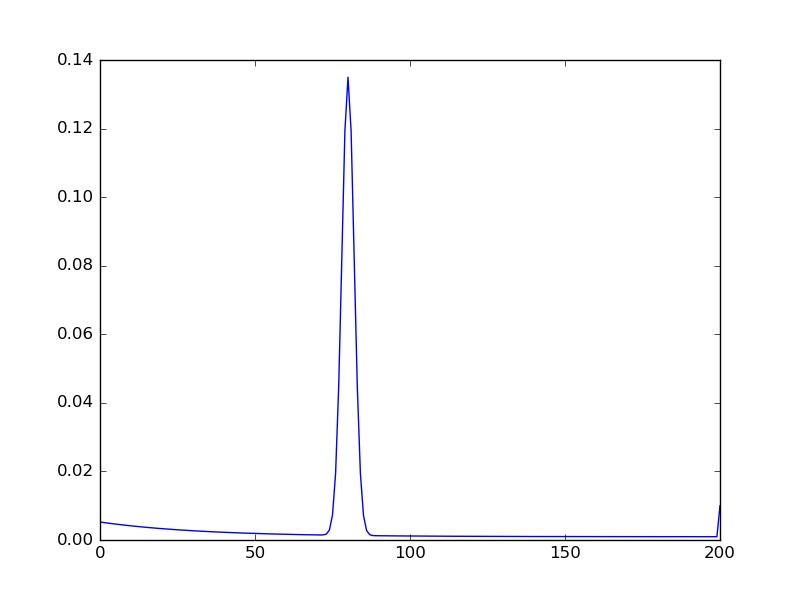
\includegraphics[width=\textwidth]{sensor_model_5.png}
  \caption{Mean 80}
 \end{minipage}
 \hfill
 \begin{minipage}[b]{0.4\textwidth}
  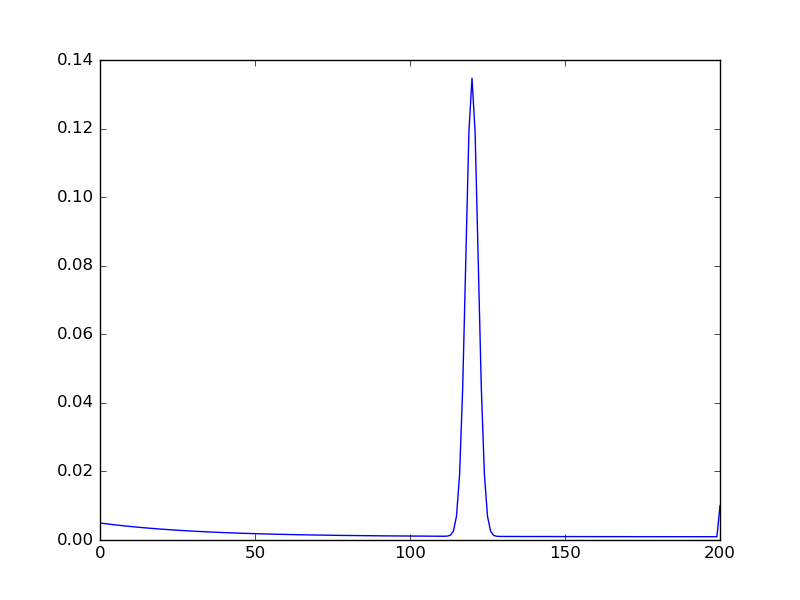
\includegraphics[width=\textwidth]{sensor_model_7.png}
  \caption{Mean 120}
 \end{minipage}
 \vfill
 \begin{minipage}[b]{0.4\textwidth}
  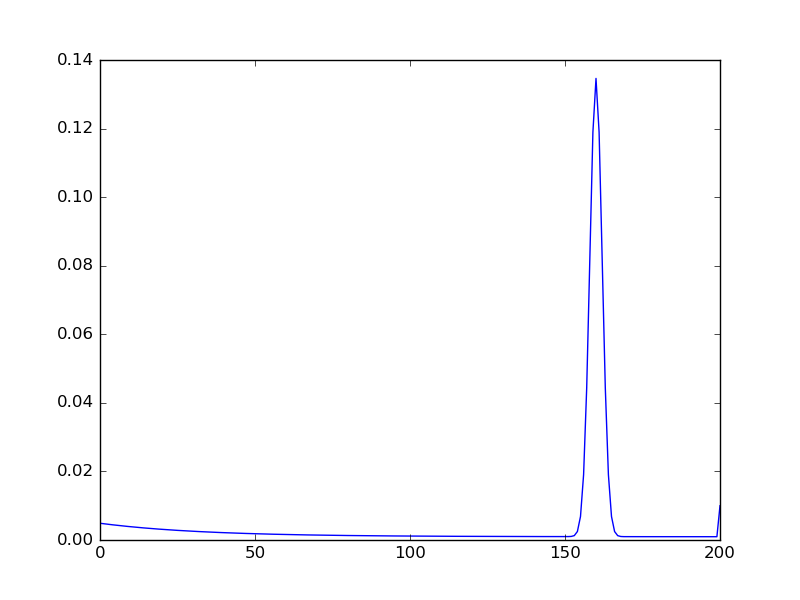
\includegraphics[width=\textwidth]{sensor_model_9.png}
  \caption{Mean 160}
 \end{minipage}
 \hfill
 \begin{minipage}[b]{0.4\textwidth}
  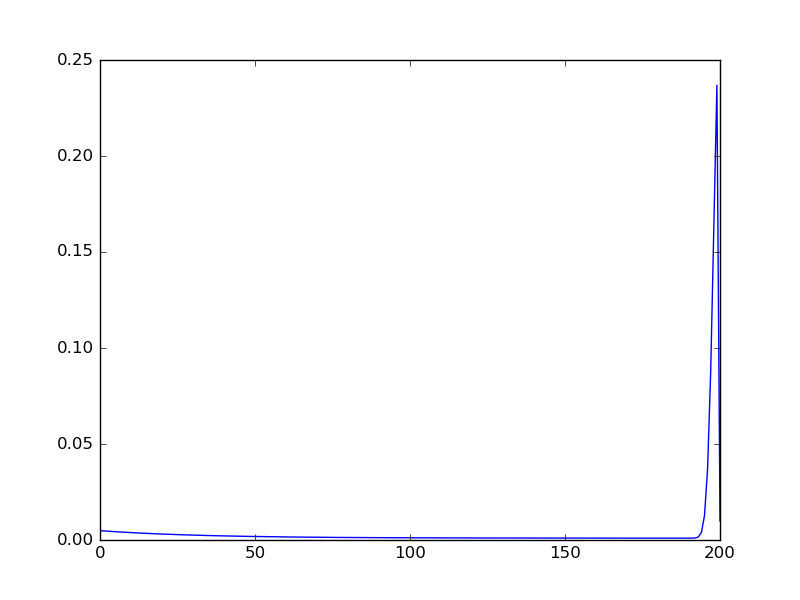
\includegraphics[width=\textwidth]{sensor_model_11.png}
  \caption{Mean 200}
 \end{minipage}

\end{figure}

\section{Extra Credit}

\subsection{Kidnapped Robot}

For extra credit, we have implemented a robust version of the particle filter which we call \textbf{doctoring}. This technique helps the localizaton algorithm by considering alternative hypothesis, and latch on to a better hypothesis, if one exists.
We resample the particles in two special cases:
\begin{enumerate}
 \item The total number of unique particles in the system goes below 20\% of the original number of particles.
 \item We maintain a randomly generated time epoch: in the range 25-45. When this epoch is reached, if the variance along x and y axis is very low (ie the particles have completely localized), we resample and generate new particles.
\end{enumerate}

The new set of random particles (\textit{num\_particles}) generated are given a weight of 1. The already existing particles are assigned a weight of 3. Now we select \textit{num\_particles} from this pool. Thus, the already existing particles are three times more likely to be selected. At this point, all the weights of all particles are reset and the particle filter restarts.

An example of the use of this algorithm can be seen in the submitted video file vid\_merged\_14.mov. Here, the particle filtering algorithm
has been run on a log obtained by fusing log1 and log4. At 1:12 mark, the robot turns into a room which signals the end of log1. At this point, log4 begins causing the number of particles in the filter to drop below 20\% based on weights assigned by the sensor model.
The \textbf{doctoring algorithm} kicks in and we can observe the robot being localized at its new position immediately after.\\


\subsection{Adaptive number of particles}
In order to analyze the effect of number of particles, we've created a video ( vid\_varying\_particles.mov ) showing the different localizations
based on the number of particles. The number of particles is shown at the top. From the video, it can be seen that after ~5000 particles,
the algorithm always localizes to the same starting position. To balance correctness and speed of the algorithm, we chose 8000 particles in
our final filtering algorithm.


\end{document}
